% !TEX encoding = UTF-8
% !TEX TS-program = pdflatex
% !TEX root = ../tesi.tex

%**************************************************************
\chapter{Azzurra Flow Engine}
\label{cap:flow engine}
%**************************************************************
\intro{Nel seguente capitolo verrà illustrato prima di tutto la struttura di un flusso conversazionale e successivamente il funzionamento del Azzurra Flow Engine la conseguente generazione dei messaggi da parte del bot Azzurre e dell'utente umano}\\

%*************************************************************

\section{Scopo}
Un elemento cardine dell'architettura di \textbf{Azzurra.flow} è \textbf{Azzurra Engine}. È un motore conversazionale in grado di ricevere in input dei flussi di conversazione i quali sono implementati attraverso file JSON, che risiedono nel database di \textbf{Azzurra.io}. Essi vengono mandati in input a \textbf{Azzurra Engine} quando il bot \textbf{Azzurra} ne fa richiesta. Questi file sono codificati secondo una certa sintassi fatta dai cosiddetti \textsf{blocchi conversazionali} i quali verranno illustrati in seguito. Tornando su \textbf{Azzurra Engine} come detto, riceve il file di conversazione in JSON in input e grazie ai metodi che ha disposizione è in grado di interpretare i file JSON ricevuti e generare i messaggi che il bot \textbf{Azzurra} deve fare visualizzare all'utente nella chat.

\section{Flussi di conversazione}
I flussi di conversazione sono degli elementi fondamentali per la conversazione tra il bot e l'utente umano. Essi sono delle configurazioni JSON, dove ogni configurazione JSON contiene un flusso di conversazione, e ogni flusso è un possibile ramo di conversazione che può essere fatto tra il bot Azzurra e l'utente umano. Ogni configurazione JSON contiene perciò dei particolari comandi che permettono al bot di sapere quali messaggi deve mostrare all'utente umano e come comportarsi in base alle sue scelte. Ogni configurazione JSON ha un \textbf{id} che contiene un codice univoco in modo tale da poter identificare ogni flusso di conversazione. Inoltre, l'esecuzione dei flussi di conversazione prevede che all'inizio ci sia l'esecuzione di un cosiddetto main flow, in modo simile a come avviene per i programmi software, cioè c'è una funzione detta main che viene eseguita per prima all'avvio del programma. Per indicare quale tra l'insieme dei flussi sia il main si utilizza il campo \textbf{isMainFlow} dandogli il valore \textsf{true}.
Oltre a questi campi esistono altri campi che sono:
\begin{itemize}
	\item \textbf{Shortcuts "shortcuts"};
	\item \textbf{Configurazione "config"};
	\item \textbf{Blocchi per la conversazione "blocks"}.
\end{itemize}
Tutti e tre verranno illustrati nelle seguenti sottosezioni.
\subsection{Shortcuts “shortcuts”}
Il campo \textbf{shortcuts} è il campo dedicato per le cosiddette "scorciatoie" cioè, nelle funzionalità che il bot offre all'utente c'è anche la possibilità di visualizzare un menu dove vengono mostrate tutte le funzionalità offerte dal bot e scegliere direttamente quelle eseguire in ogni momento.

\begin{figure}[htbp]
	\centering
	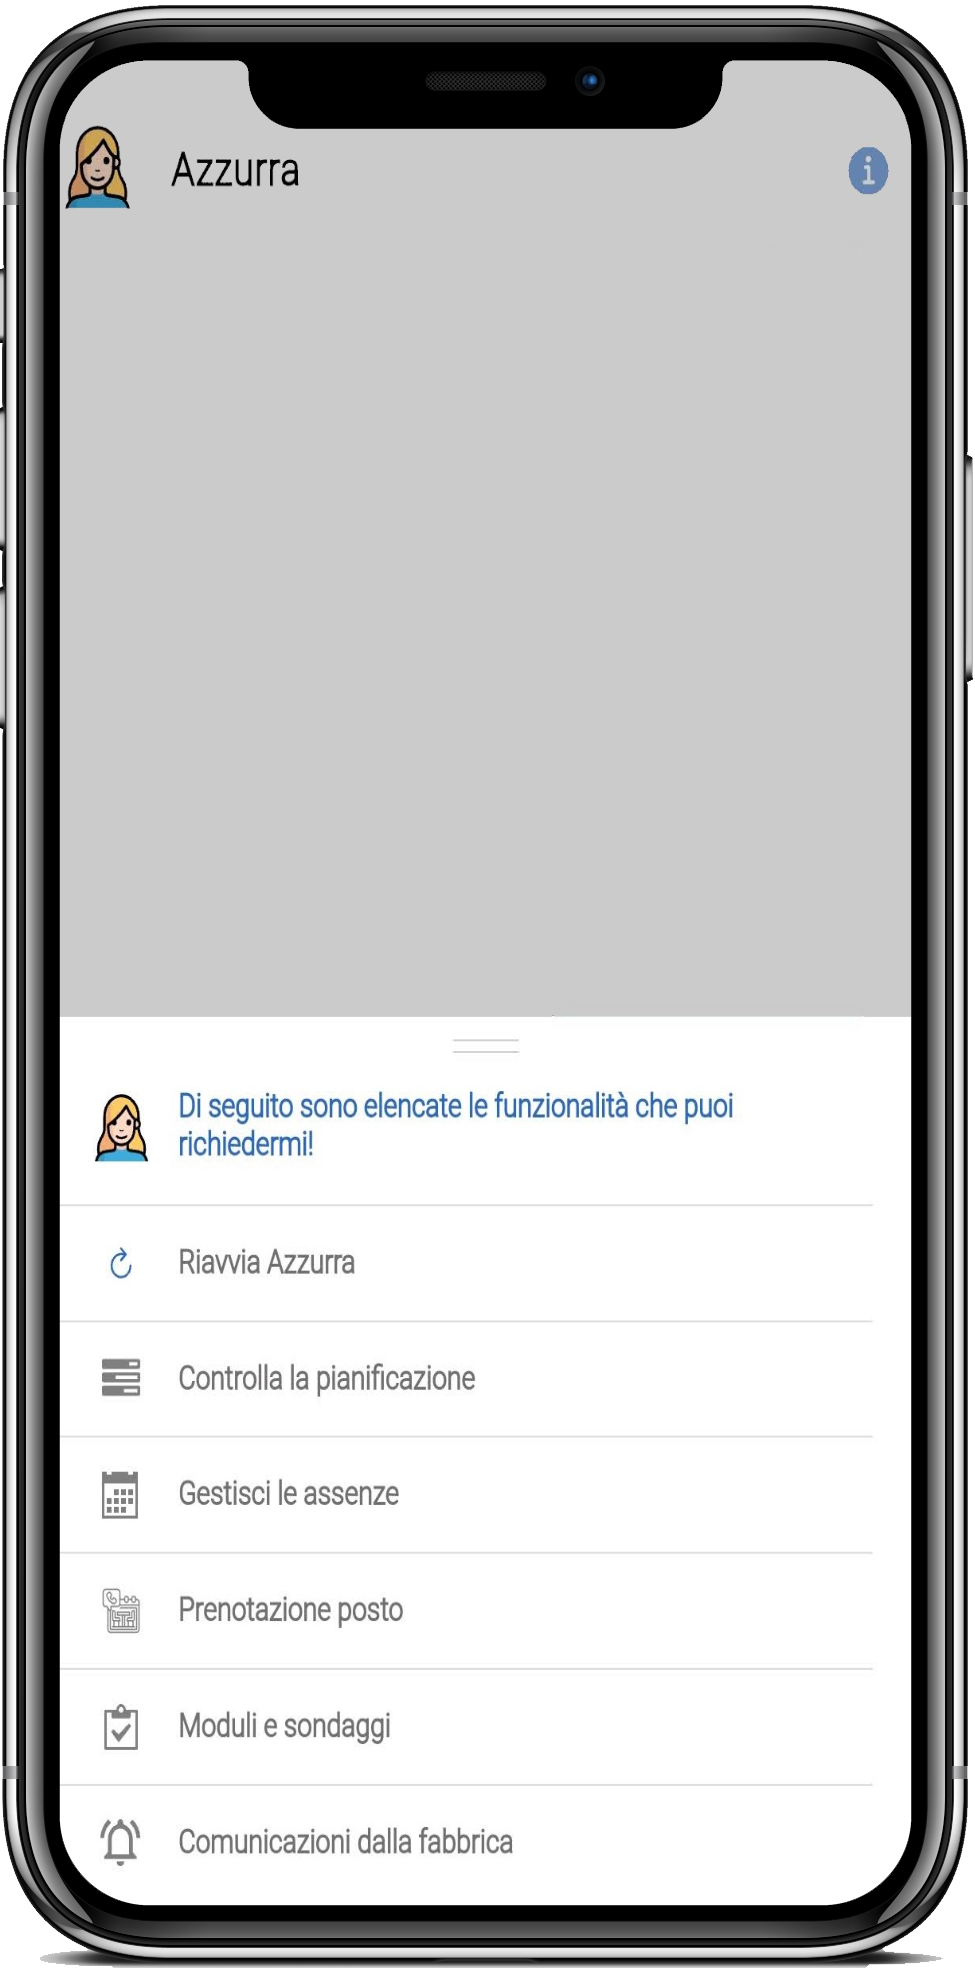
\includegraphics[scale=0.4]{shortcuts.PNG}
	\caption{Menu contenente le shortcuts disponibili}
\end{figure}

Il campo \textbf{shortcuts} viene indicato nel file con la keyword \textbf{shortcuts}
e al suo interno contiene i seguenti campi:
\begin{itemize}
	\item \textbf{text}: È un campo che può essere di tipo \textsl{string} contenente il testo da far visualizzare nel bottone della scorciatoia all'utente, oppure un oggetto che contiene un attributo per ogni lingua disponibile. Il testo nella lingua di default (italiano) è contenuto nell’attributo “default” ;
	\item \textbf{flowId}: Contiene l'identificativo del flusso che la scorciatoia permette di far eseguire;
	\item \textbf{icon}: Per rendere la UI più accattivante è possibile aggiungere al bottone dedicato alla scorciatoia, delle icone per ogni scorciatoia.
\end{itemize}
\clearpage
\subsection{Configurazione "config"}
Il campo \textbf{config} permette di indicare attraverso il campo \textbf{startBlockId} quale blocco di conversazione del flusso deve essere eseguito per primo, per tale campo ci sarà il codice identificativo del primo blocco da eseguire. Il campo \textbf{configurazione} viene indicato nel file con la keyword \textbf{config}.

\subsection{Blocchi per la conversazione}
Il campo \textbf{Blocchi} indicato nel file con la keyword \textbf{blocks} contiene tutti i blocchi per la conversazione i quali indicano quali messaggi devono essere mostrati e quali operazioni eseguire a seconda delle scelte inserite dell'utente umano.
I blocchi utilizzati per la conversazione si differenziano tra lo loro dal tipo di blocco a cui appartengono. Ogni tipo ha proprie caratteristiche uniche ma anche delle caratteristiche comuni questo perché tutti i tipi di blocchi per la conversazione ereditano da un tipo padre detto \textbf{BLOCK}. I tipi figli di \textbf{Block} sono i seguenti:
\begin{itemize}
	\item\textbf{ASK};
	\item\textbf{SAY};
	\item\textbf{IF};
	\item\textbf{PROC};
	\item\textbf{JUMP};
	\item\textbf{CALLFUNC}.
\end{itemize}
Di seguito verrà illustrata la struttura del tipo e il ruolo di \textbf{BLOCK} e dei suoi figli.
\subsubsection{BLOCK}

Il blocco \textbf{BLOCK} come detto è il blocco di conversazione attraverso il quale tutti blocchi ereditano delle caratteristiche comuni della loro struttura, di fatto il blocco \textbf{BLOCK} non può essere utilizzato è quindi può essere paragonato a una classe astratta nell'ambito della programmazione ad oggetti, dove vengono definite delle caratteristiche della classe ma non può essere istanziata, perciò può essere solo ereditata dai suoi figli, che diventano classi concrete istanziabili.

%\begin{figure}[htbp]
%	\centering
%	\includegraphics[height=5cm]{img/block.png}
%	\caption{Definizione della classe BLOCK}
%\end{figure}

Ha la seguente struttura:

\begin{itemize}
	\item \textbf{id}: È un campo di tipo \textsl{string} il quale identifica univocamente il blocco tra un insieme di blocchi di conversazione;
	\item \textbf{type}: Questo campo indica il tipo di blocco che come detto può essere di tipo \textbf{ASK} o \textbf{SAY} o \textbf{IF} o \textbf{PROC} o \textbf{JUMP} oppure \textbf{CALLFUNC};        
	\item \textbf{text}: È un campo che può essere di tipo \textsl{string} contente il testo da far visualizzare all'utente, oppure un oggetto che contiene un attributo per ogni lingua disponibile contente del testo nella corrispondente lingua, e un attributo default che contiene il testo di default;
	\item \textbf{variations}: Anch'esso è un tipo \textsl{string} che contiene uno o più testi alternati al principale rappresentato dal campo \textbf{text}. Il funzionamento prevede che randomicamente il testo da mostrare all'utente non sarà quello principale ma uno delle alternative contenuto all'interno di \textbf{variations}, verrà perciò scelto in modo casuale, uno dei testi a disposizione; 
	\item \textbf{target}: Questo campo contiene l'id del prossimo blocco di conversazione da eseguire;
	\item \textbf{variable}: Questo campo indica il nome della variabile su cui salvare eventuali valori di input inseriti dall'utente; \\
	Percio, il flow engine attraverso i suoi metodi, ha la capacità di salvare tutte le scelte fatte dell'utente, memorizzandole nelle variabili indicate nel campo \textbf{variable}.
	\item \textbf{widget}: Indica il tipo di oggetto grafico detto \textsf{Widget} che deve essere utilizzato a supporto del blocco, esisto i seguenti tipi di \textsf{Widget}:
	\begin{itemize}
		\item \textbf{BUTTONS};
		\item \textbf{ITEMS};
		\item \textbf{PICKER};
		\item \textbf{TIMEPICKER};
		\item \textbf{DATEPICKER};
		\item \textbf{CALENDAR};
		\item \textbf{QRSCANNER}.
	\end{itemize}
	Più avanti verranno illustrati in dettaglio;
	\item \textbf{widgetOptions}:Permette di aggiungere delle opzioni in più al \textsf{Widget} per esempio permette di indicare del testo all'interno dei \textsf{Widget} oppure indicare il valore minimo accettabile.
\end{itemize} 


\subsubsection{ASK}
Il blocco di conversazione \textbf{ASK} ha la funzione di mostrare all'utente una serie di opzioni disponibili e chiedere quali tra queste vuole eseguire. Quindi mostra le opzioni definite precedentemente all'utente, rimane in attesa di una risposta dell'utente e infine esegue la scelta effettuata dall'utente. 

%\begin{figure}[htbp]
%	\centering
%	\includegraphics[scale=0.7] {img/ask.png}
%	\caption{Definizione della classe ASK}
%\end{figure}

Oltre a campi del tipo \textbf{BLOCK} ha i seguenti campi in più:

\begin{itemize}
	\item \textbf{category}: Il blocco \textbf{ASK} è ulteriormente distinguibile in \textsf{ASK} o in \textsf{MENU} che si differenziano nel seguente aspetto:\\
	nel caso sia di categoria \textsf{ASK} tutte le opzioni disponibili portano a un blocco di conversazione successivo diverso mentre per \textsf{MENU} tutte le opzioni portano tutte allo stesso blocco;
	\item \textbf{source}: Parametro che contiene il nome di una variabile a cui fare riferimento per prendere i dati da utilizzare, se non si fa riferimento a nessuna variabile allora va settato a \textsf{NULL};
	\item \textbf{items}: Questo campo contiene un array d'oggetti di tipo \textsl{BlockItem} che rappresentano le possibile scelte che può fare l'utente, essi graficamente vengono rappresentati come dei pulsanti;
	\item \textbf{sourceType}: Parametro che indica la modalità di utilizzo della variabile contenuta nel campo \textbf{source};
	Ci sono solo due modalità disponibili:
	\begin{itemize}
		\item \textbf{LIST}: In questo caso la variabile contenuta in \textbf{source} viene ignorata e vengono presi tutti gli oggetti di tipo \textsl{BlockItem} contenuti nel campo \textbf{items} che vengono trasformati in bottoni da far visualizzare a video;
		\item \textbf{VARIABLE}: In questo caso tutto ciò che è contenuto nella variabile del campo \textbf{source} viene trasformato in bottoni da far visualizzare a video, per poterlo fare devono essere formattati in una struttura del tipo chiave valore.
	\end{itemize}	
\end{itemize} 

\subsubsection{SAY}

Il blocco di conversazione \textbf{SAY} ha la funzione di mostrare all'utente un messaggio a video attraverso il quale si comunica l'esito della operazione precedente e il risultato da essa ricavata. Perciò l'utente richiede l'esecuzione di una qualche operazione, viene eseguita e una volta conclusa il bot risponderà all'utente con il risultato ricavato precedentemente.

%\begin{figure}[htbp]
%	\centering
%	
\includegraphics[scale=0.7]{img/say.png}
%	\caption{Definizione della classe SAY}
%\end{figure}
Oltre a campi del tipo \textbf{BLOCK} ha il seguente campo in più:

\begin{itemize}
	\item \textbf{attachment}: Campo che contiene un array d'oggetti di tipo \textsl{BlockAttachment} che permettono di allegare immagini o file PDF.
\end{itemize}

Inoltre sono presenti i campi \textbf{items}, \textbf{source} e \textbf{sourceType}, con analogo funzionamento del blocco \textbf{ASK} per inserire eventuali bottoni che aprono schede o link contenenti il risultato richiesto.

\subsubsection{IF}

Il blocco di conversazione \textbf{IF} ha la funzione di verificare se una o più condizioni sono rispettate. Perciò verifica se le condizioni sono soddisfatte se sì farà un certo tipo di operazioni previste, se invece non sono soddisfatte si eseguiranno altre operazioni.

%\begin{figure}[htbp]
%	\centering
%	\includegraphics[scale=1]{img/if.png}
%	\caption{Definizione della classe IF}
%\end{figure}
Oltre a campi del tipo \textbf{BLOCK} ha i seguenti campi in più:

\begin{itemize}
	\item \textbf{conditions}: Contiene una o più condizioni che devono essere verificate;
	\item \textbf{trueBlockTarget}: Indica il blocco successivo da eseguire se le condizioni sono soddisfate;
	\item \textbf{falseBlockTarget}: Indica il blocco successivo da eseguire se le condizioni non sono soddisfate.
\end{itemize}


\subsubsection{PROC}
Il blocco di conversazione \textbf{PROC} permette di eseguire delle operazioni sulle variabili conversazionali quali assegnazione o trasformazione di dato. Ad esempio, permette di riordinare i dati ricevuti dal server in modo da poter essere utilizzati dai \textbf{source} con \textbf{sourceType} uguale a \textbf{VARIABLE}.

%\begin{figure}[htbp]
%	\centering
%	\includegraphics[scale=1]{img/proc.png}
%	\caption{Definizione della classe PROC}
%\end{figure}

Oltre a campi del tipo \textbf{BLOCK} ha il seguente campo in più:

\begin{itemize}
	\item \textbf{expressions}: Contiene le espressioni da eseguire, ad esempio, per la formattazione dei dati.
	Ha i seguenti campi:
	\begin{itemize}
		\item \textbf{var}: Contiene il nome della variabile dove viene salvato il risultato della formattazione;
		\item \textbf{type}: Indica il tipo di formattazione che si vuole applicare, al momento c'è solo una formattazione disponibile:
		\begin{itemize}
			\item \textbf{reduce to textvalue}: Permette di riordinare i vari valori che si hanno in una struttura chiave valore.
		\end{itemize}
		\item \textbf{args}: Contiene un espressione in \textsf{Handlebars}, un linguaggio di templating utilizzato per costruire template in HTML con dei cosiddetti segnaposto che verranno poi valorizzati con dei valori, utilizzando delle keyword del linguaggio, in modo da ottenere delle componenti in HTML da mostrare come messaggio.
	\end{itemize}
\end{itemize}

\subsubsection{JUMP}

Il blocco di conversazione \textbf{JUMP} permette di cambiare il flusso di conversazione ed eseguirne una altro. In termini tecnici si passa Da un JSON di configurazione ad un altro dove ogni configurazioni JSON contiene un specifico flusso di esecuzione, grazie a \textbf{JUMP} si può "saltare" da un flusso di conversazione a un altro.

%\begin{figure}[htbp]
%	\centering
%	\includegraphics[height=5cm]{img/jump.png}
%	\caption{Definizione della classe JUMP}
%\end{figure}

Nel campo target non viene indicato l'id del blocco successivo ma, l'id del flow che si vuole eseguire.

\subsubsection{CALLFUNC}

Il blocco di conversazione \textbf{CALLFUNC} è il blocco attraverso il quale, il bot (la mobile App) può richiedere l’esecuzione di chiamate ad API (interne o esterne). Attraverso un WebSocket, che mantiene una connessione tra il bot e Azzurra.io, quest’ultima richiama, a sua volta, delle API di AWMS (o esterne ad AWMS) per ottenere i dati richiesti dell’utente o per salvare dati. 

%\begin{figure}[htbp]
%	\centering
%	\includegraphics[scale=1]{img/callfun.png}
%	\caption{Definizione della classe CALLFUNC}
%\end{figure}

Oltre a campi del tipo \textbf{BLOCK} ha il seguente campo in più:

\begin{itemize}
	\item \textbf{payload}: Campo che contiene l'intestazione e il corpo della richiesta verso Azzurra.io;
	Contiene i seguenti campi:
	\begin{itemize}
		\item \textbf{type}: Indica se la chiamata è verso Azzurra.io attraverso il valore \textsf{int} oppure verso un servizio esterno con il valore \textsf{ext}.
	\end{itemize}
	Se la chiamata è di tipo \textsf{int} ha la seguente struttura:
	\begin{itemize}
		\item \textbf{route}: Indica il metodo di Azzurra.io da richiamare ;
		\item \textbf{body}: Contiene il corpo della richiesta, nello specifico un template costruito da \textsf{Handlebars} che verrà idratato da Azzurra.io nel caso sia una richiesta di dati o dal bot nel caso in cui debba inviare dei dati da salvare.
	\end{itemize}
	Se la chiamata è di tipo \textsf{ext} ha la seguente struttura:
	\begin{itemize}
		\item \textbf{config}: Contiene la struttura di una chiamata HTTP.\\
		Ha i seguenti campi:
		\begin{itemize}
			\item \textbf{url}: Contiene l'indirizzo URL del servizio esterno a cui fare richiesta;
			\item \textbf{method}: Se la richiesta e di tipo \textsf{GET} o \textsf{POST};
			\item \textbf{headers}: Contiene l'intestazione per la richiesta HTTP;
			\item \textbf{params}: Contiene le variabili necessarie per la chiamata, questo campo viene usato solo se il la richiesta e di tipo \textsf{GET};
			\item \textbf{data}: Analogo al campo \textbf{params} solo che viene usato dai metodi POST.
		\end{itemize}
	\end{itemize}
	\item \textbf{var}: Indica il nome della variabile dove salvare il risultato della richiesta;
	\item \textbf{failureBlockTarget}: Indica il blocco successivo da eseguire se la richiesta non va a buon fine;
	\item \textbf{successBlockTarget}: Indica il blocco successivo da eseguire se la richiesta va a buon fine.
\end{itemize}

\subsection{Oggetti ausiliari}
Come detto nella sezione precedente questi oggetti vengono definiti per poterli utilizzarli all'interno dei blocchi per svolgere un azione di supporto ai blocchi affinché si possa raggiungere ciò per cui sono stati realizzati i blocchi di conversazione stessi.\\
\\
Di seguito vengono indicate tutte le classi degli oggetti ausiliari disponibili.

\subsubsection*{Widget}
È un oggetto che a seconda del tipo permette di realizzare delle componenti grafiche, esso viene utilizzo per richiedere delle azioni da parte dell’utente umano.
Ha i seguenti tipi:
\begin{itemize}
	\item \textbf{BUTTONS}: Genera dei bottoni arrotondati;
	\item \textbf{ITEMS}: Genera dei bottoni quadrati;
	\item \textbf{PICKER}: Genera attraverso l'\textsf{ion-picker} di \textsf{Ionic} una finestra di dialogo dove si può selezionare una opzione tra quelle proposte;
	\item \textbf{TIMEPICKER}: Analogo al \textbf{PICKER} solo che le opzioni da scegliere e l'orario che si vuole selezionare;
	\item \textbf{DATEPICKER}: Analogo al \textbf{PICKER} solo che le opzioni da scegliere e la data che si vuole selezionare;
	\item \textbf{CALENDAR}: Fa comparire un calendario grazie all'utilizzo del plugin \textsf{Calendar} per \textsf{Ionic};
	\item \textbf{QRSCANNER}: Permette di accedere alla fotocamera (solo se si hanno i permessi) e leggere i codici \textsf{QR-code} tutto ciò grazie al plugin \textsf{QR Scanner} per \textsf{Ionic}.
\end{itemize}

\subsubsection*{BlockItem}
Questo oggetto rappresenta una possibile scelta che può fare l'utente, graficamente viene rappresentato come un bottone cliccabile dall'utente.
Ha la seguente struttura:

\begin{itemize}
	\item \textbf{text}: Contiene l'etichetta che viene visualizzata sul bottone;
	\item \textbf{target}: Contiene l'id del prossimo blocco da eseguire.
\end{itemize}

\subsubsection*{BlockAttachment} 
L'oggetto in esame permette di allegare immagini o file PDF da mostrare all'utente.

Ha la seguente struttura:

\begin{itemize}
	\item \textbf{id}: Contine un codice univoco che identifica ogni \textsl{BlockAttachment};
	\item \textbf{type}: Indica se contiene un PDF o una immagine, nel caso di un'immagine indica se è in formato \textsf{JPG} o in \textsf{JPEG} oopure in \textsf{PNG}.
\end{itemize}	
